\section{Results}
\label{sec:results}
\subsection{Data}
The proposed novel consensus model is applied to the selection,
average and rank $3$ model. The CSD model got replaced by the rank $3$ model
because it was knocked off compared to the other models by Dice score. Further,
the CSD used in the model is computational heavy, i.e. computation takes 4 times as long
as the $4$th order CSD which is used within this paper. This especially matters
because of the time intense bootstrap creation. 

To evaluate the proposed models, data from the Human
Connectome Project (HCP) is used \cite{HCP}. The diffusion MR images have a resolution of $1.25$ mm
isotropic with $145 \times 174 \times 145$ voxels. 

As reference data we use the high quality data, which was published within the
scope of the Tractseg paper \cite{WASSERTHAL2018239}. This reference data has been
created by manually refining the segmented full brain fiber tractography. For
more details we refer to the original literature.

All tests were performed on 12 randomly chosen subjects for which such reference tractographies
exist. For each tract we created seed points by intersecting the reference
fiber bundle with a plane and initialize the tracking process with the direction
of the fiber bundle at the seed point. This should mimic a directional region of
interest as it might be defined by an expert on brain anatomy
\cite{Graumann2016}. We then apply the tracking process until we have as many
streamlines as the reference tractography. This should guaranty that the
comparison between the different models is fair.

\subsection{Qualitative Comparison}
\begin{figure*}[t]
	\centering
	\begin{minipage}{0.19\linewidth}
\begin{subfigure}[b]{\linewidth}
		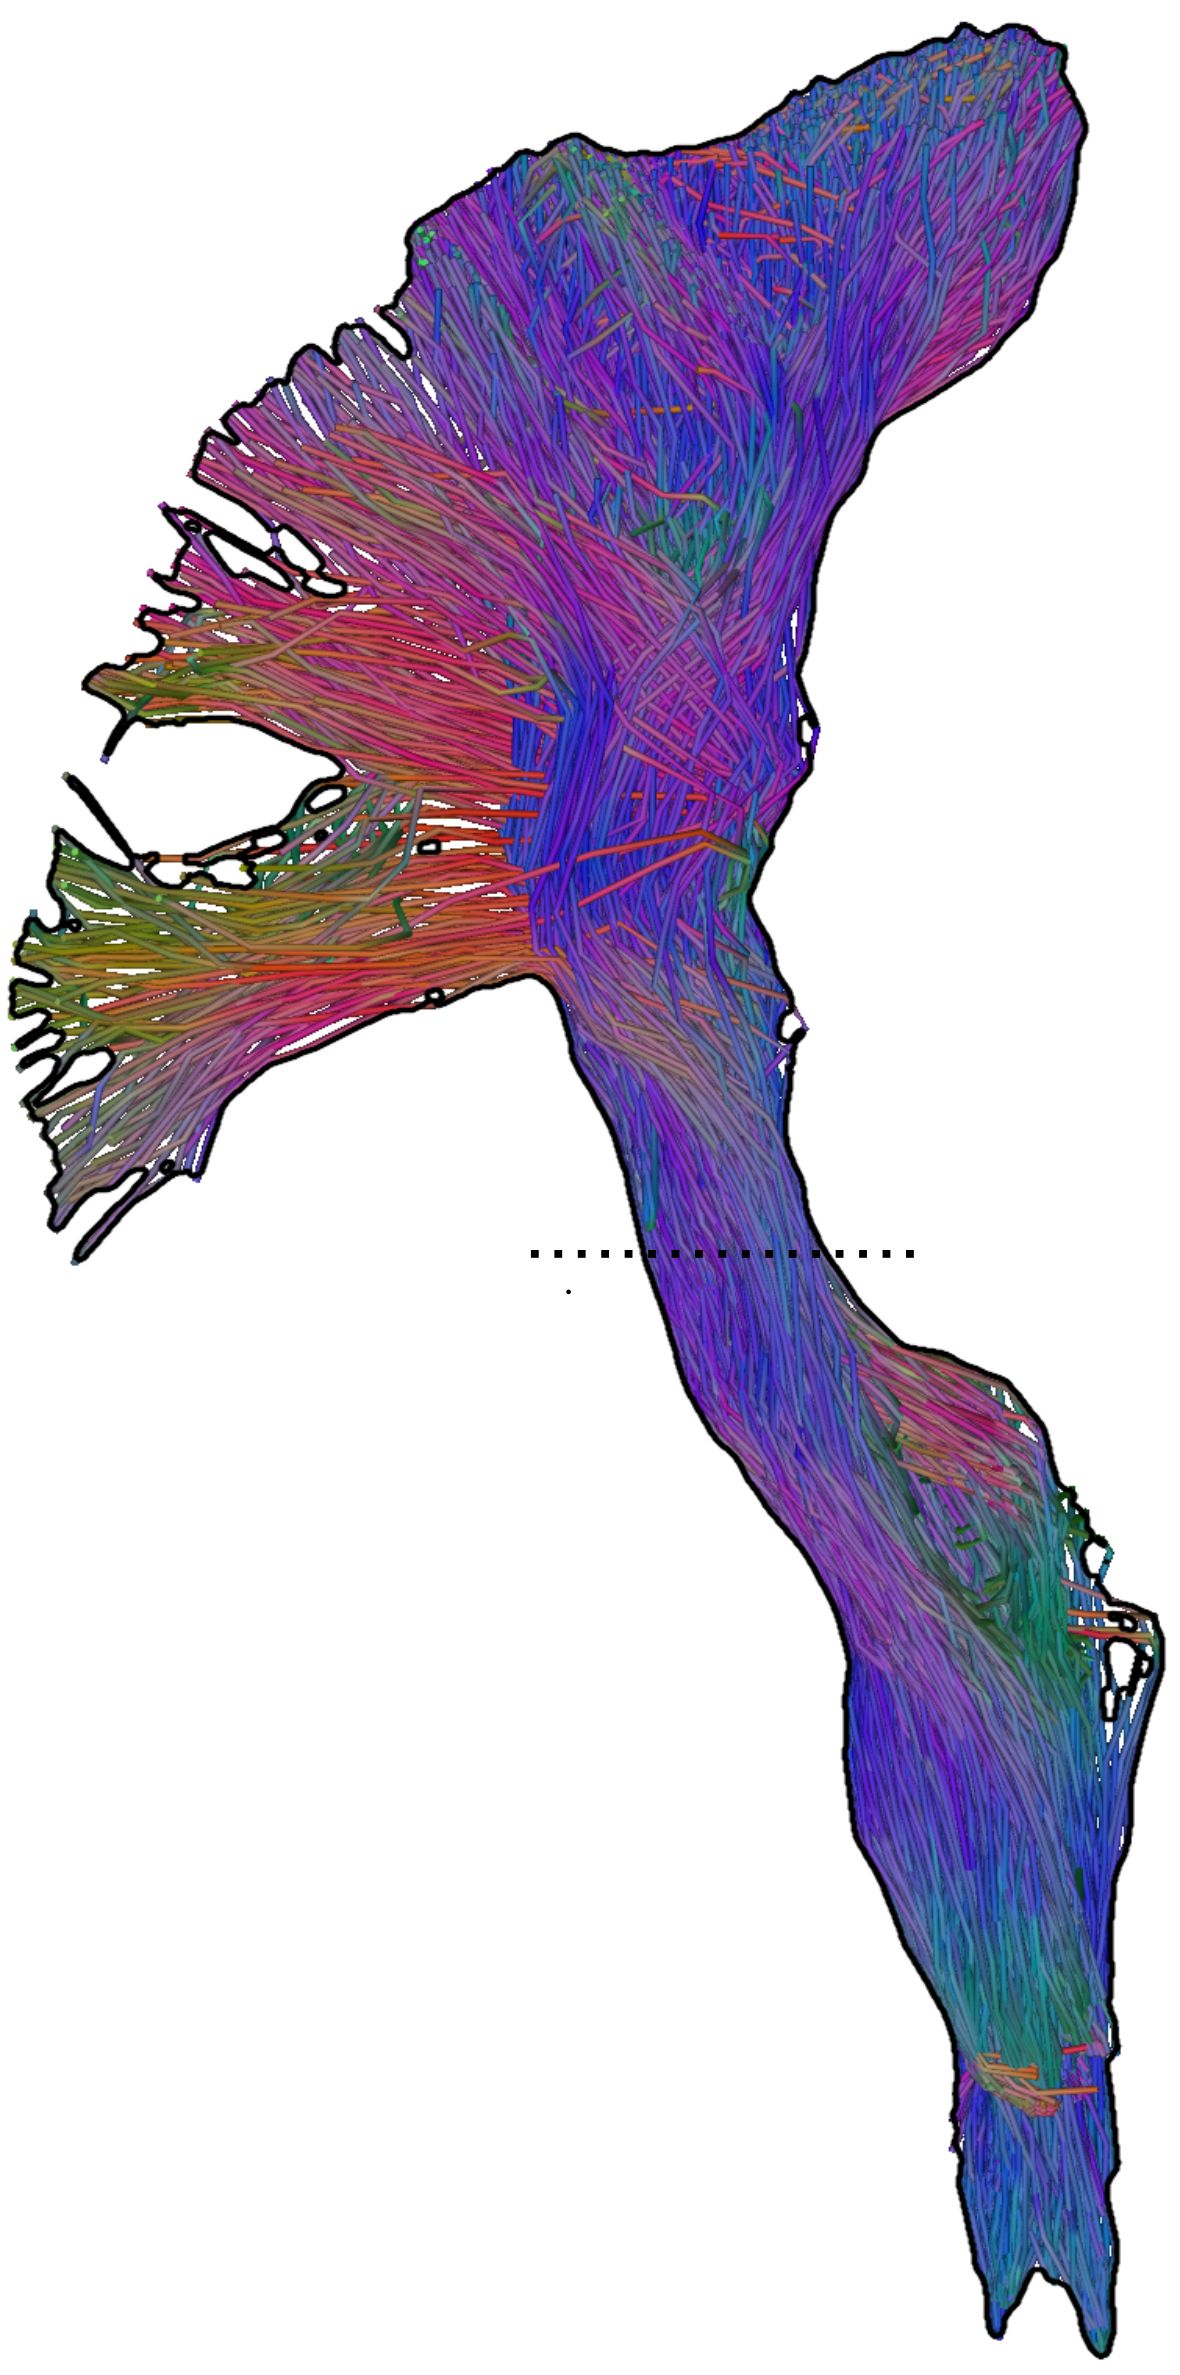
\includegraphics[width=\linewidth]{cst-ref-c}
		\caption{Low rank 3 model {\color{white} avdsdsds} }
	\end{subfigure}
\end{minipage}
\hfil
	\begin{minipage}{0.19\linewidth}
		\begin{subfigure}[b]{\linewidth}
		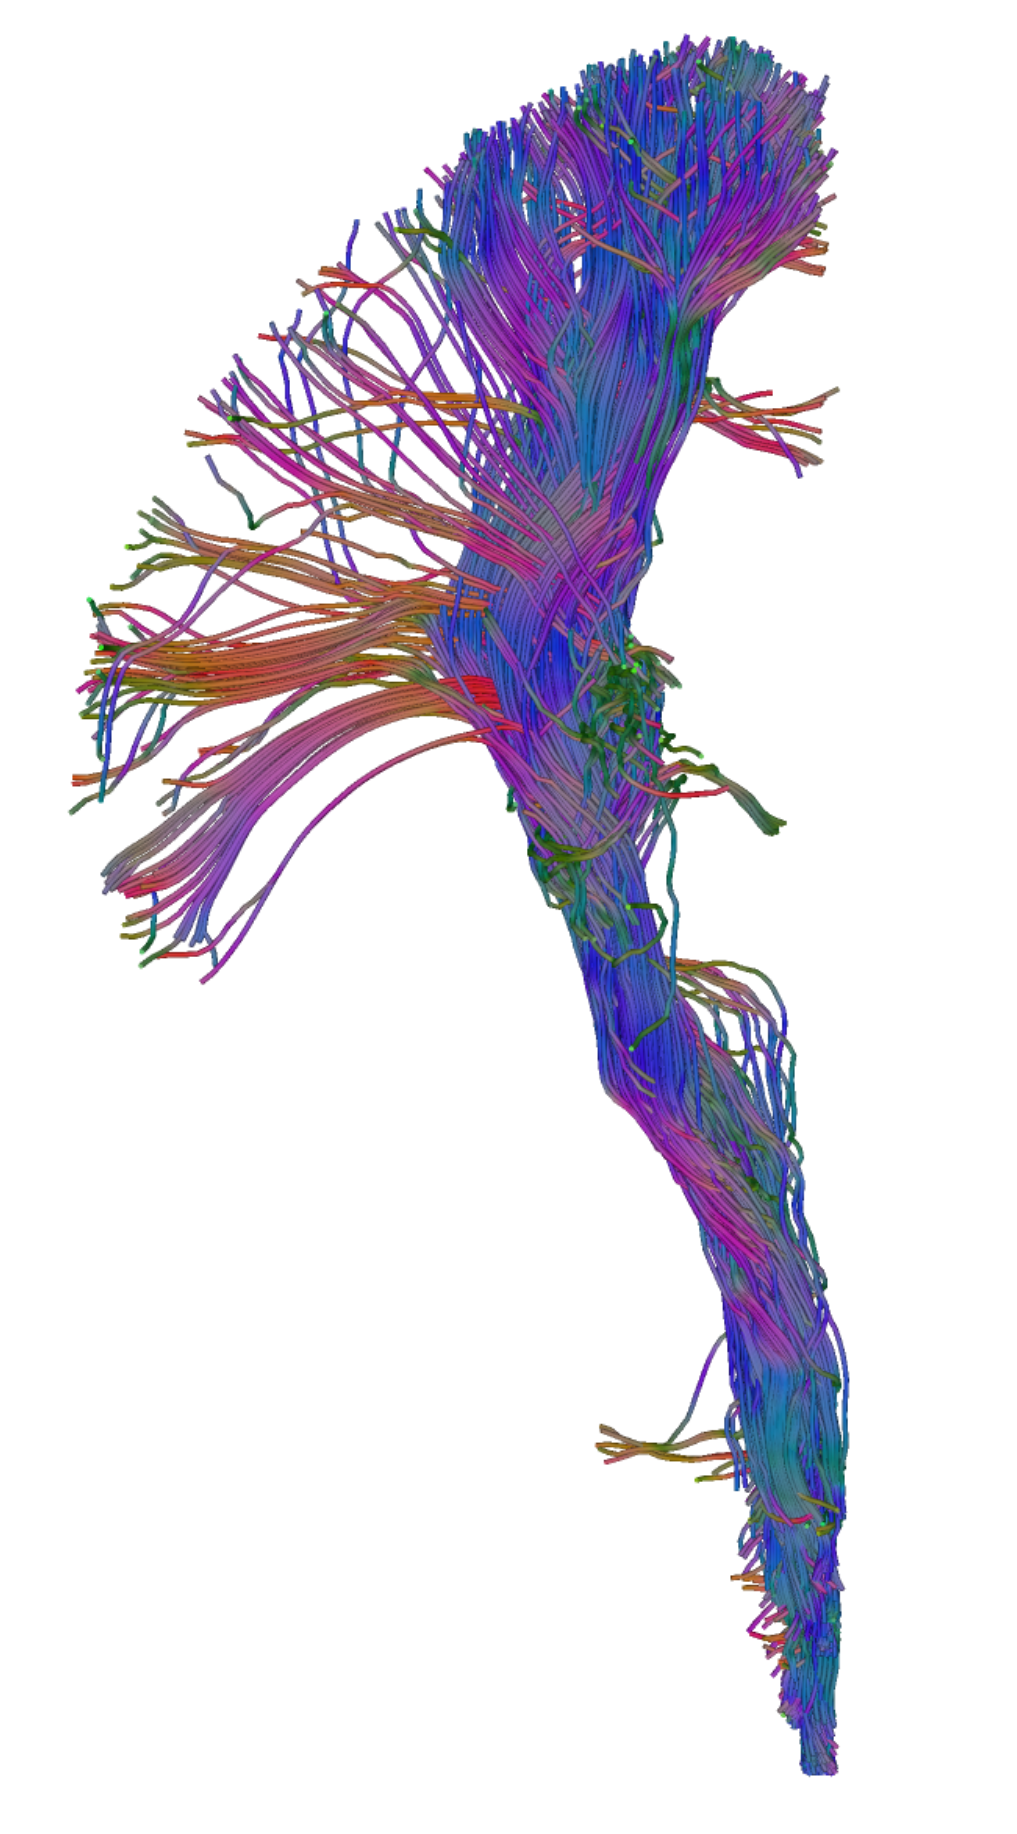
\includegraphics[width=\linewidth]{cst-rank-c}
		\caption{Low rank 3 model {\color{white} avdsdsds} }
	\end{subfigure}
	\begin{subfigure}[b]{\linewidth}
		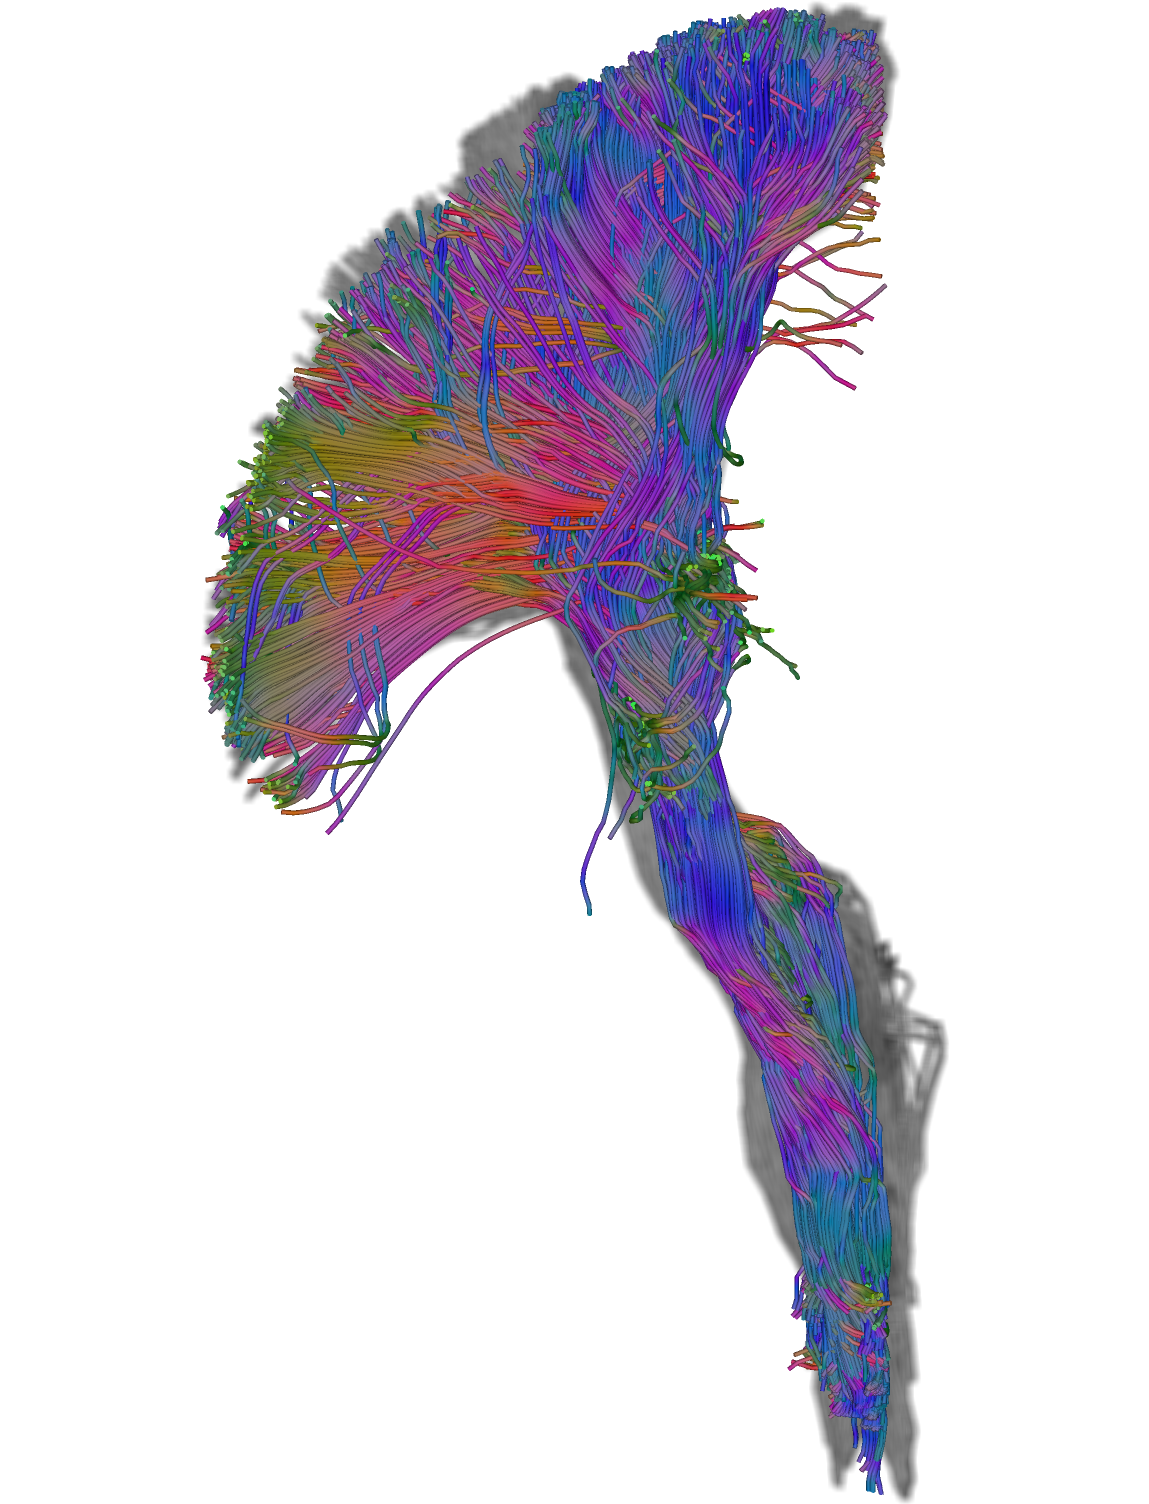
\includegraphics[width=\linewidth]{cst-rank-bootstrap-c}
		\caption{Consensus low rank 3 model}
\end{subfigure} 
	\end{minipage} \hfil
	\begin{minipage}{0.19\linewidth}
	\begin{subfigure}[b]{\linewidth}
		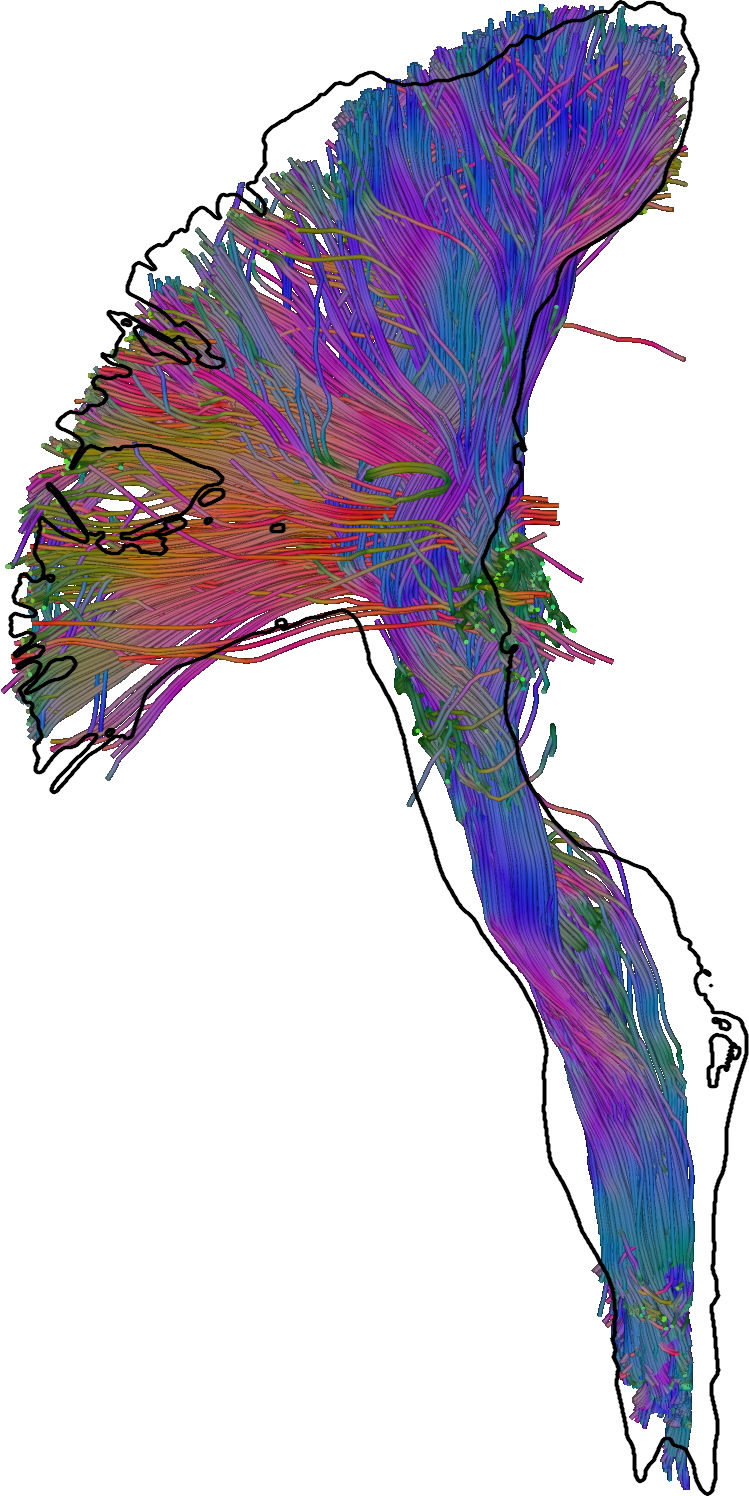
\includegraphics[width=\linewidth]{cst-avg-c}
		\caption{Average model {\color{white} aasfd vdsdsds}}
	\end{subfigure}
	\begin{subfigure}[b]{\linewidth}
		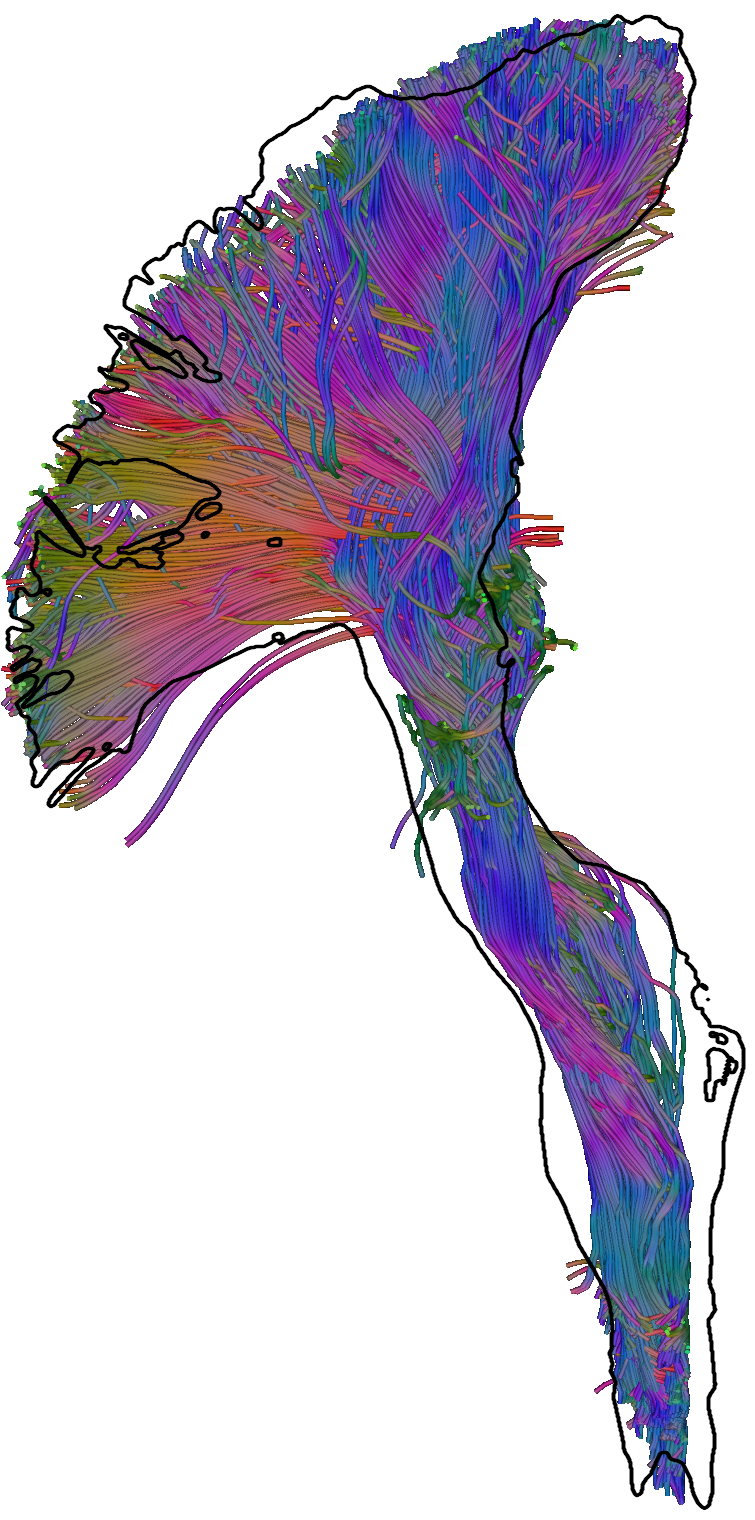
\includegraphics[width=\linewidth]{cst-avg-bootstrap-c}
		\caption{Consensus Average model{\color{white} aasfd vdsdsds}}
\end{subfigure} 
	\end{minipage} \hfil 
	\begin{minipage}{0.19\linewidth} 
	\begin{subfigure}[b]{\linewidth}
		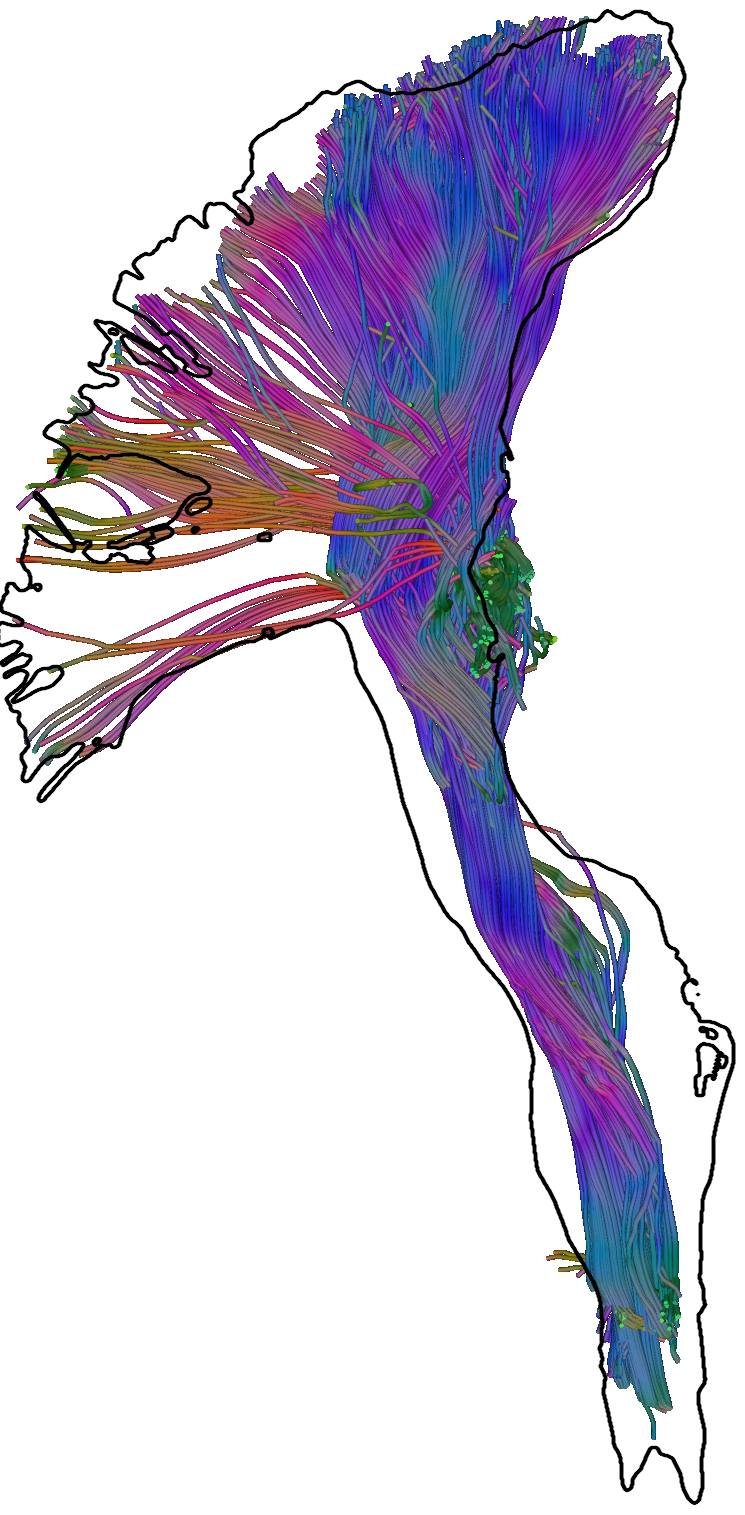
\includegraphics[width=\linewidth]{cst-sel-c}
		\caption{Selection model {\color{white} avdsdsds asdf asdf}}
	\end{subfigure}
	\begin{subfigure}[b]{\linewidth}
		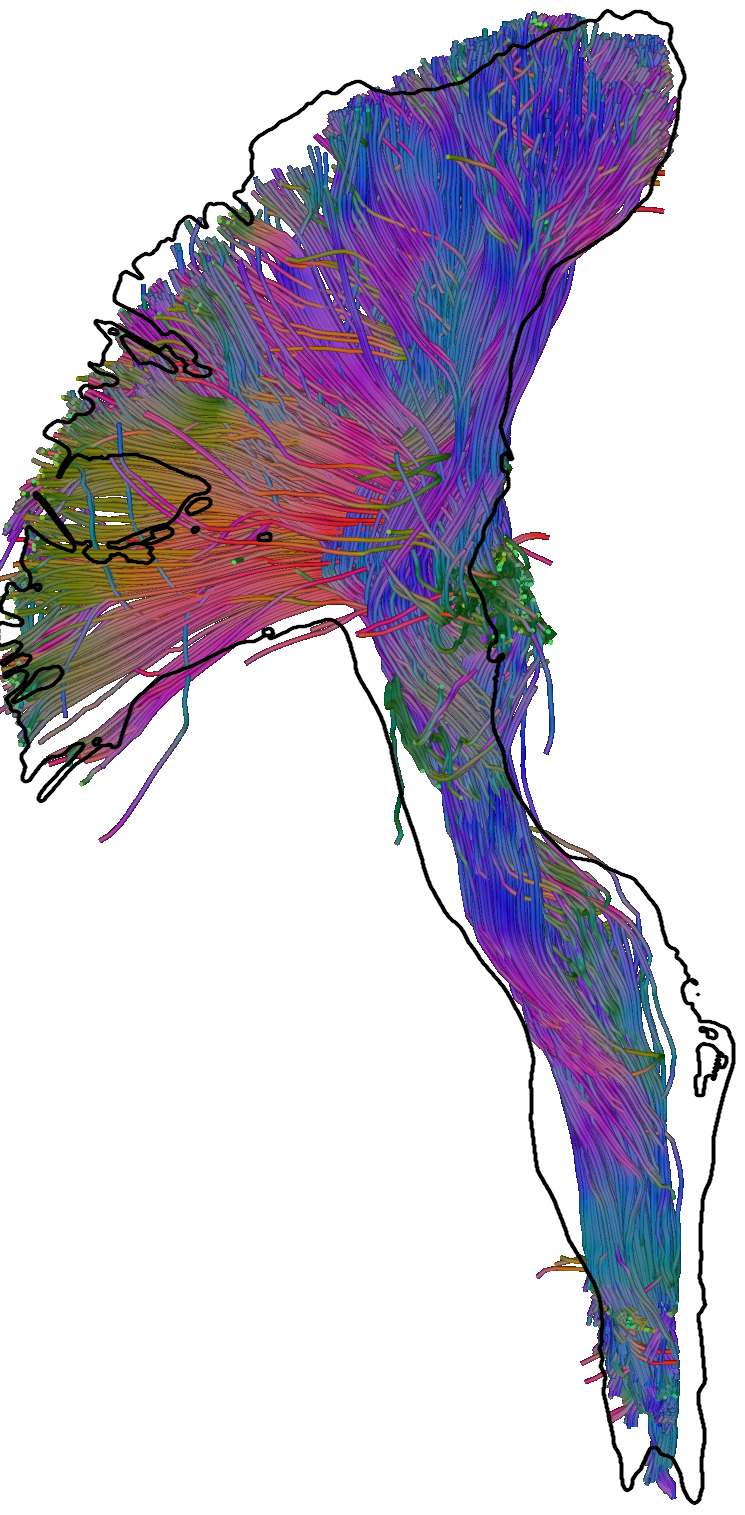
\includegraphics[width=\linewidth]{cst-sel-bootstrap-c}
		\caption{Consensus Selection Model}
\end{subfigure} 
	\end{minipage}
\caption{Reconstruction of the right Corticospinal Tract. To make the comparison
	between the reference and the tractographies more intuitive, we have
	indicated contour of the reference in each reconstruction with a black
	line. The seed region is indicated by
the black dashed line. Within the consensus models the tracking algorithm shows a much higher ability
to reconstruct the lateral spread compared to the base models. This is
especially true for the selection model, where the reconstruction in the base
model misses a lot of the lateral spread.  }
	\label{fig:CST}
\end{figure*}
\begin{figure*}[t]
	\centering
\begin{subfigure}[b]{0.23\linewidth}
		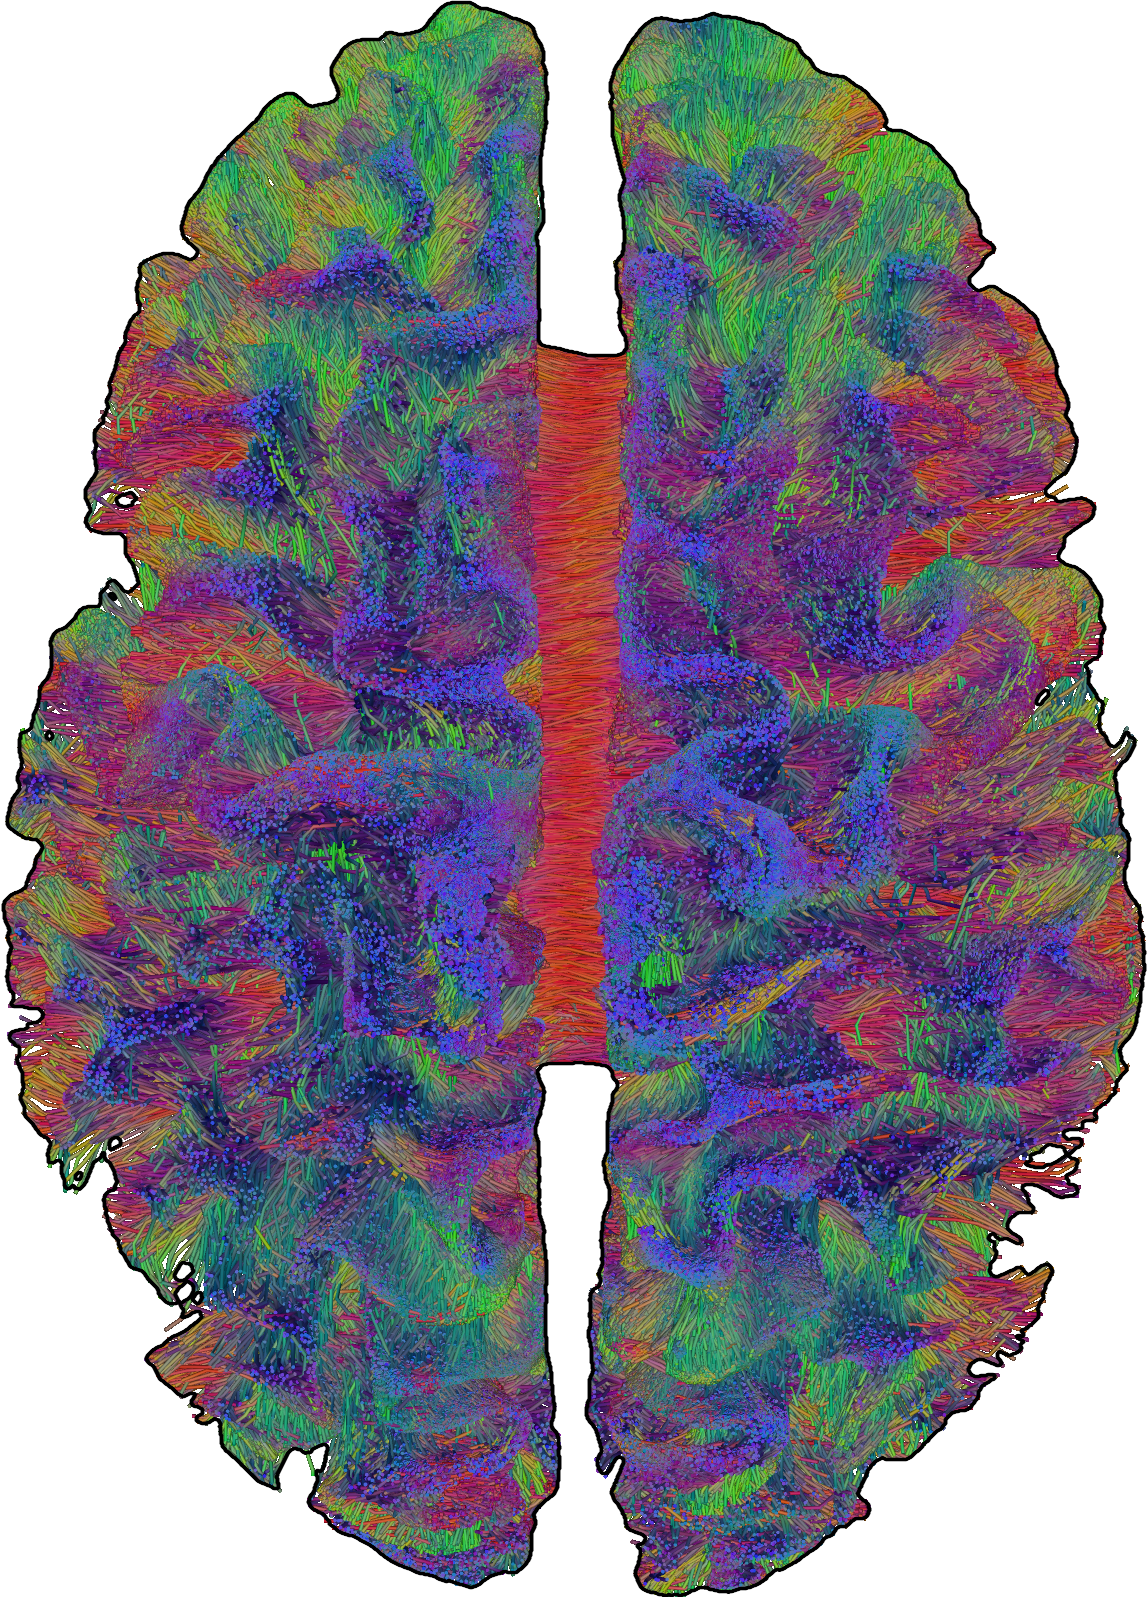
\includegraphics[width=\linewidth]{cc-ref-c}
		\caption{Low rank 3 model {\color{white} avdsdsds} }
	\end{subfigure}
	\hspace{0.01\linewidth}
	\begin{subfigure}[b]{0.23\linewidth}
		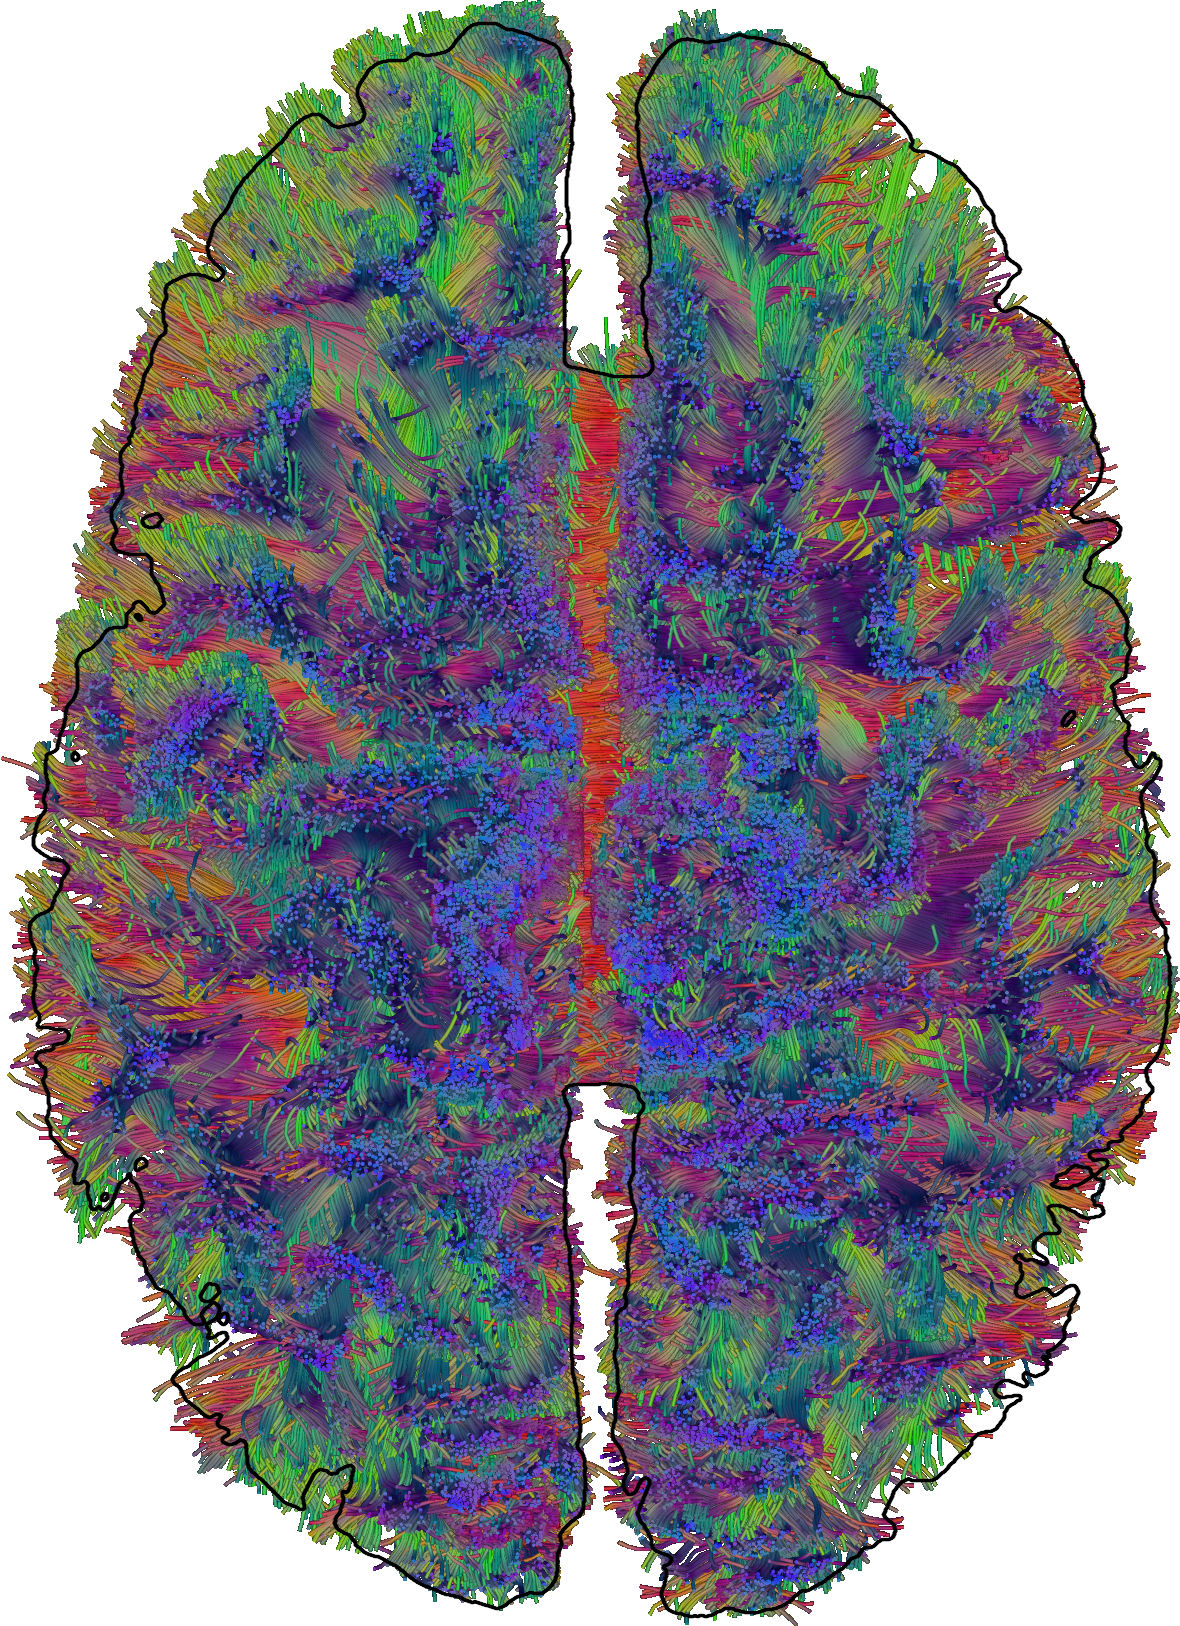
\includegraphics[width=\linewidth]{cc-rank-c}
		\caption{Low rank 3 model {\color{white} avdsdsds} }
	\end{subfigure}
	\hspace{0.01\linewidth}
	\begin{subfigure}[b]{0.23\linewidth}
		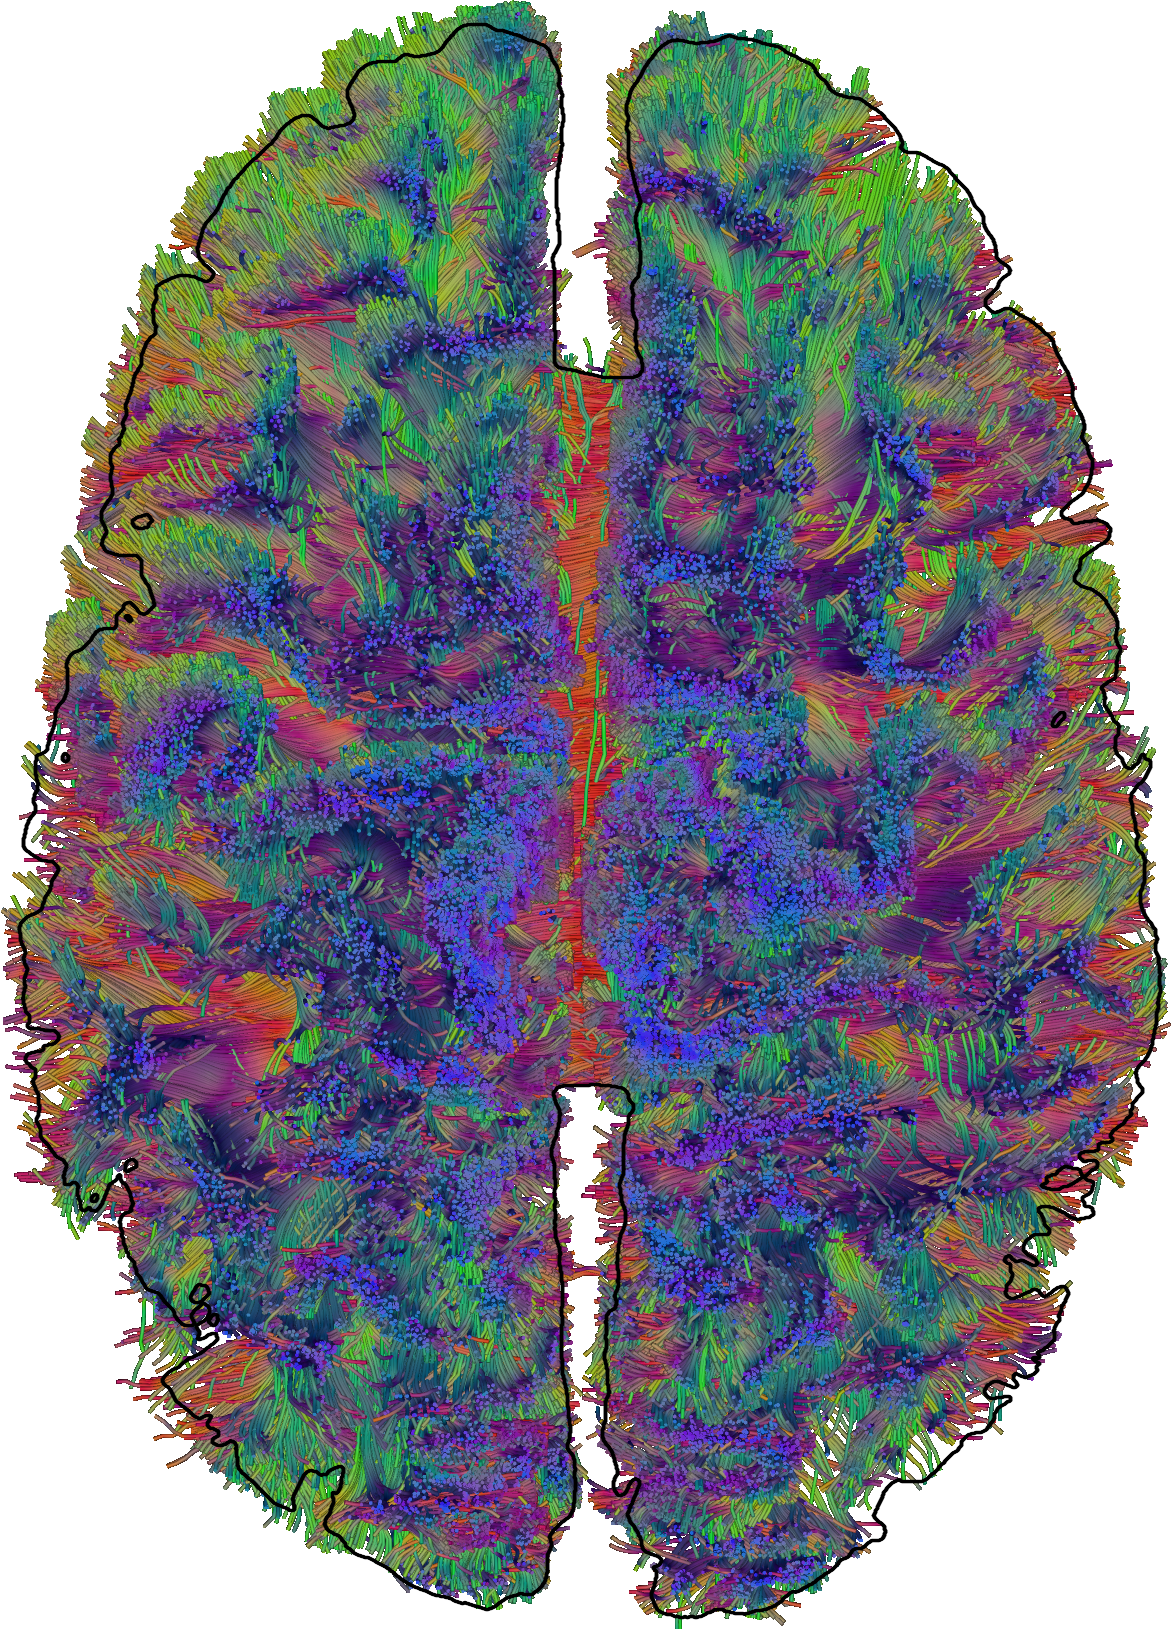
\includegraphics[width=\linewidth]{cc-rank-bootstrap-c}
		\caption{Consensus low rank 3 model}
\end{subfigure} \\ 
	\begin{subfigure}[b]{0.23\linewidth}
		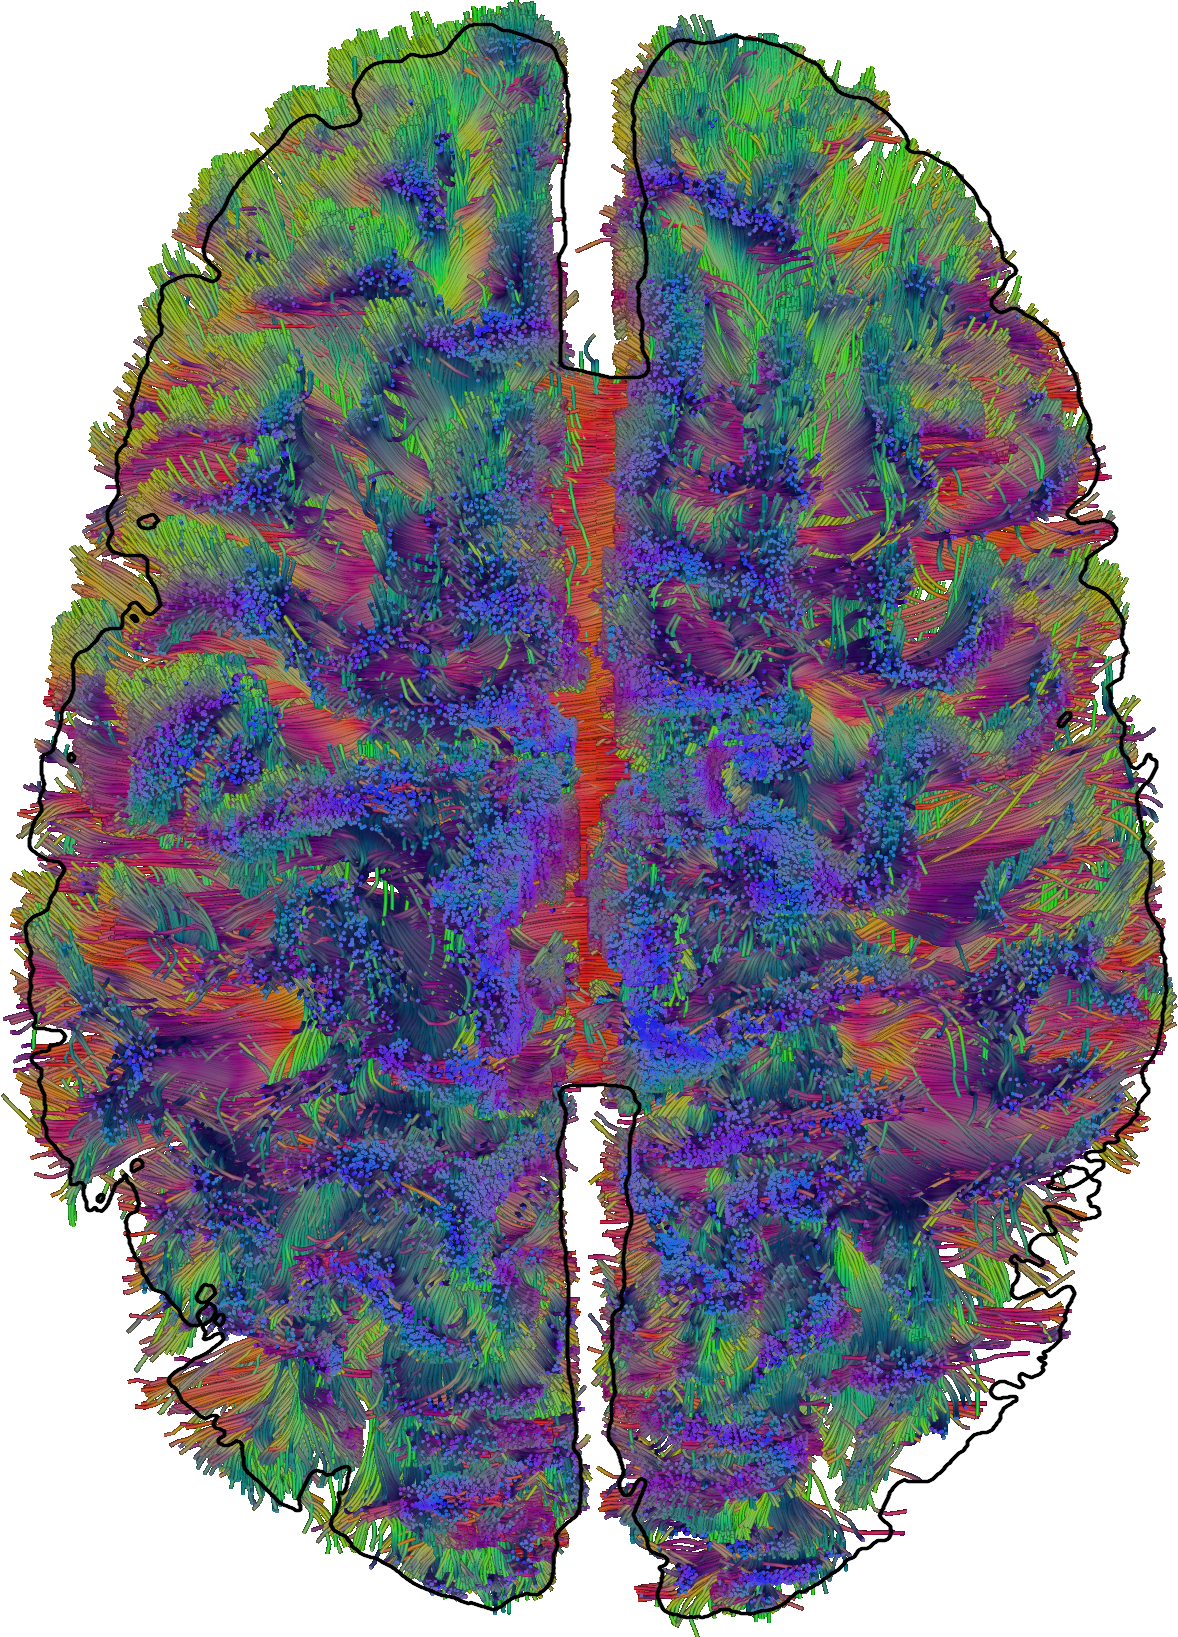
\includegraphics[width=\linewidth]{cc-avg-c}
		\caption{Average model {\color{white} avdsdsds}}
\end{subfigure} 
	\hspace{0.01\linewidth}
	\begin{subfigure}[b]{0.23\linewidth}
		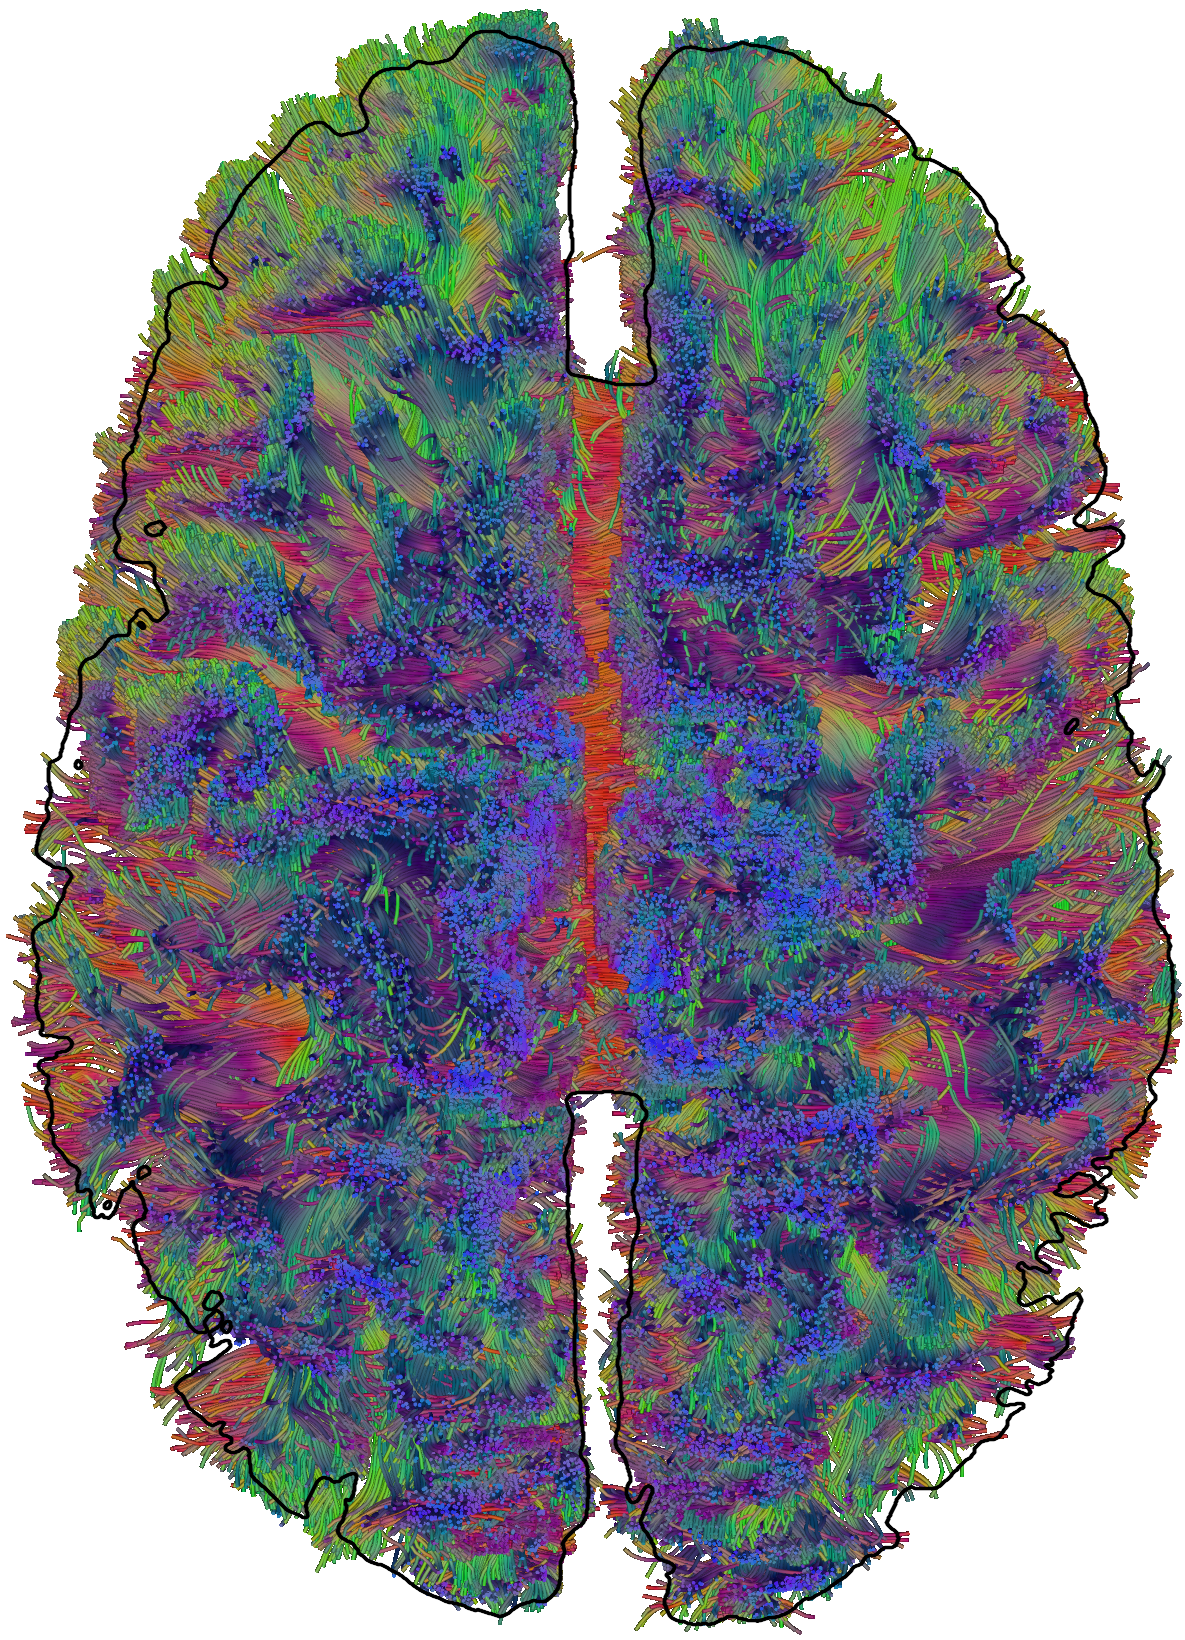
\includegraphics[width=\linewidth]{cc-avg-bootstrap-c}
		\caption{Consensus Average model}
\end{subfigure} 
	\hspace{0.01\linewidth}
\begin{subfigure}[b]{0.23\linewidth}
		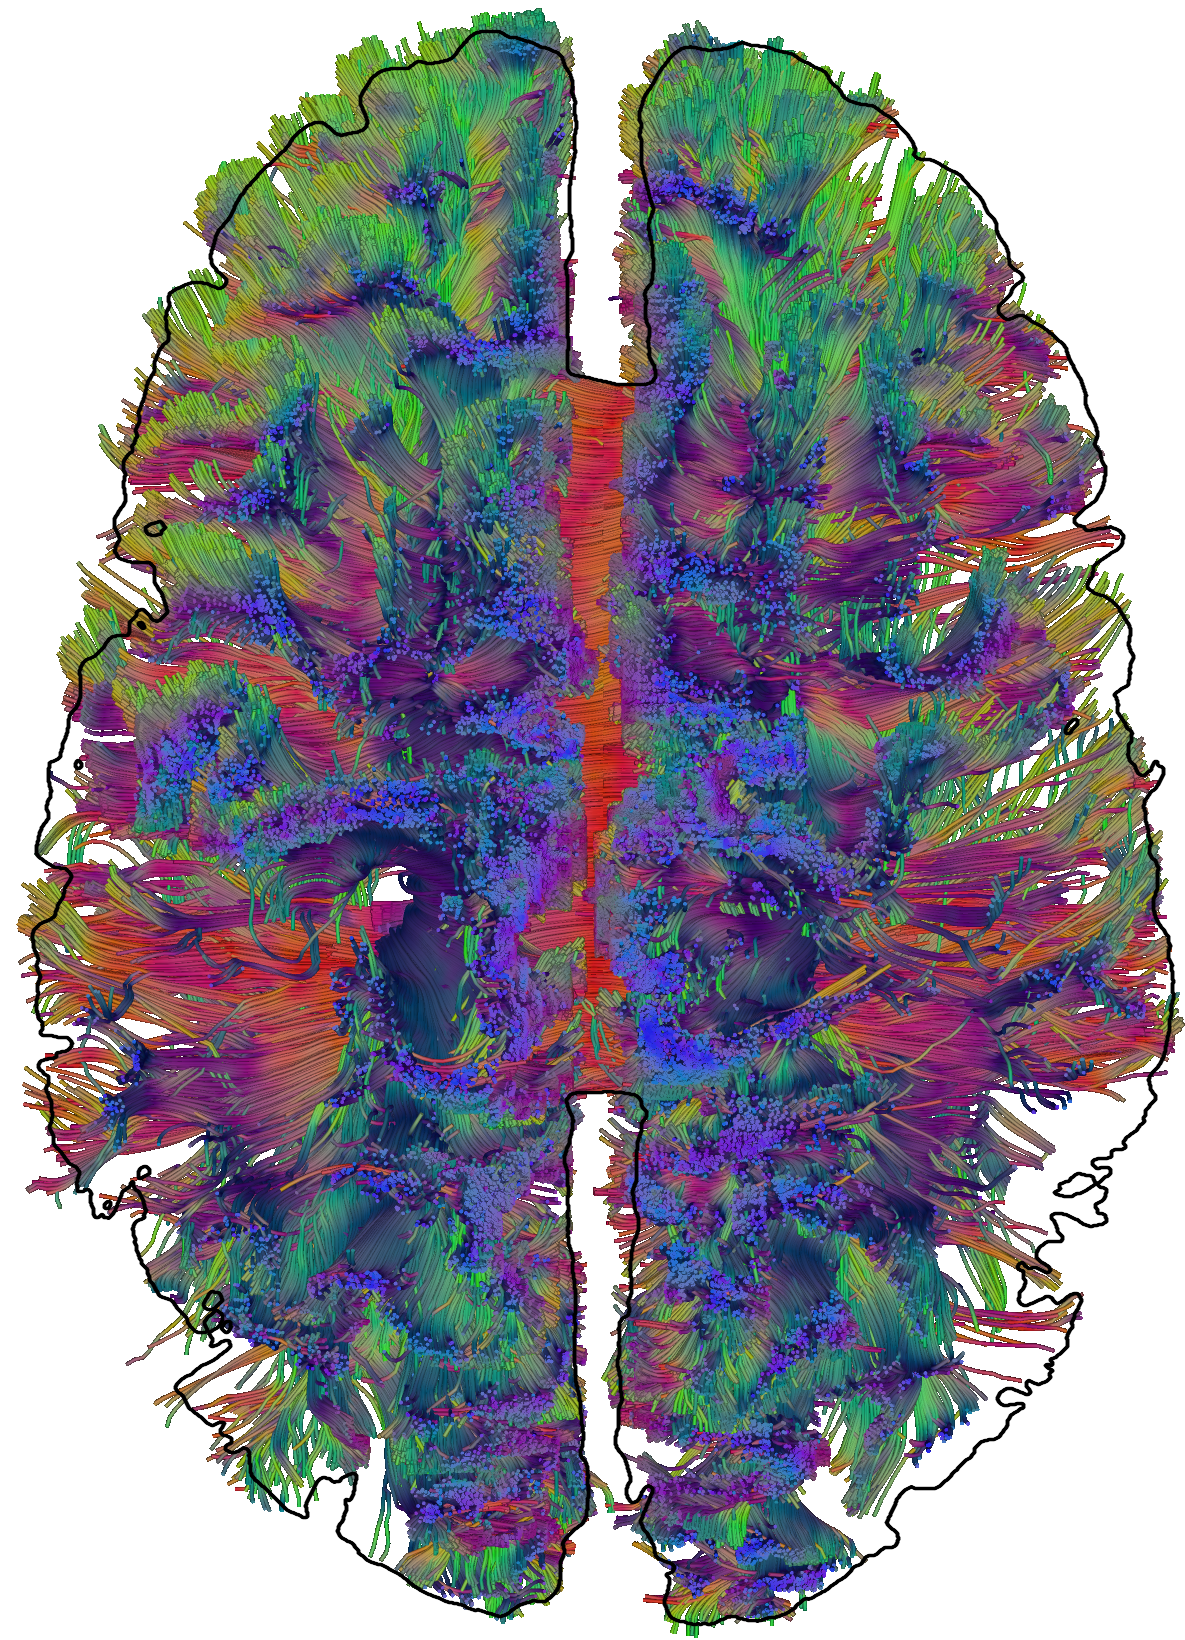
\includegraphics[width=\linewidth]{cc-sel-c}
		\caption{Selection model {\color{white} avdsdsds}}
	\end{subfigure}
	\hspace{0.01\linewidth}
	\begin{subfigure}[b]{0.23\linewidth}
		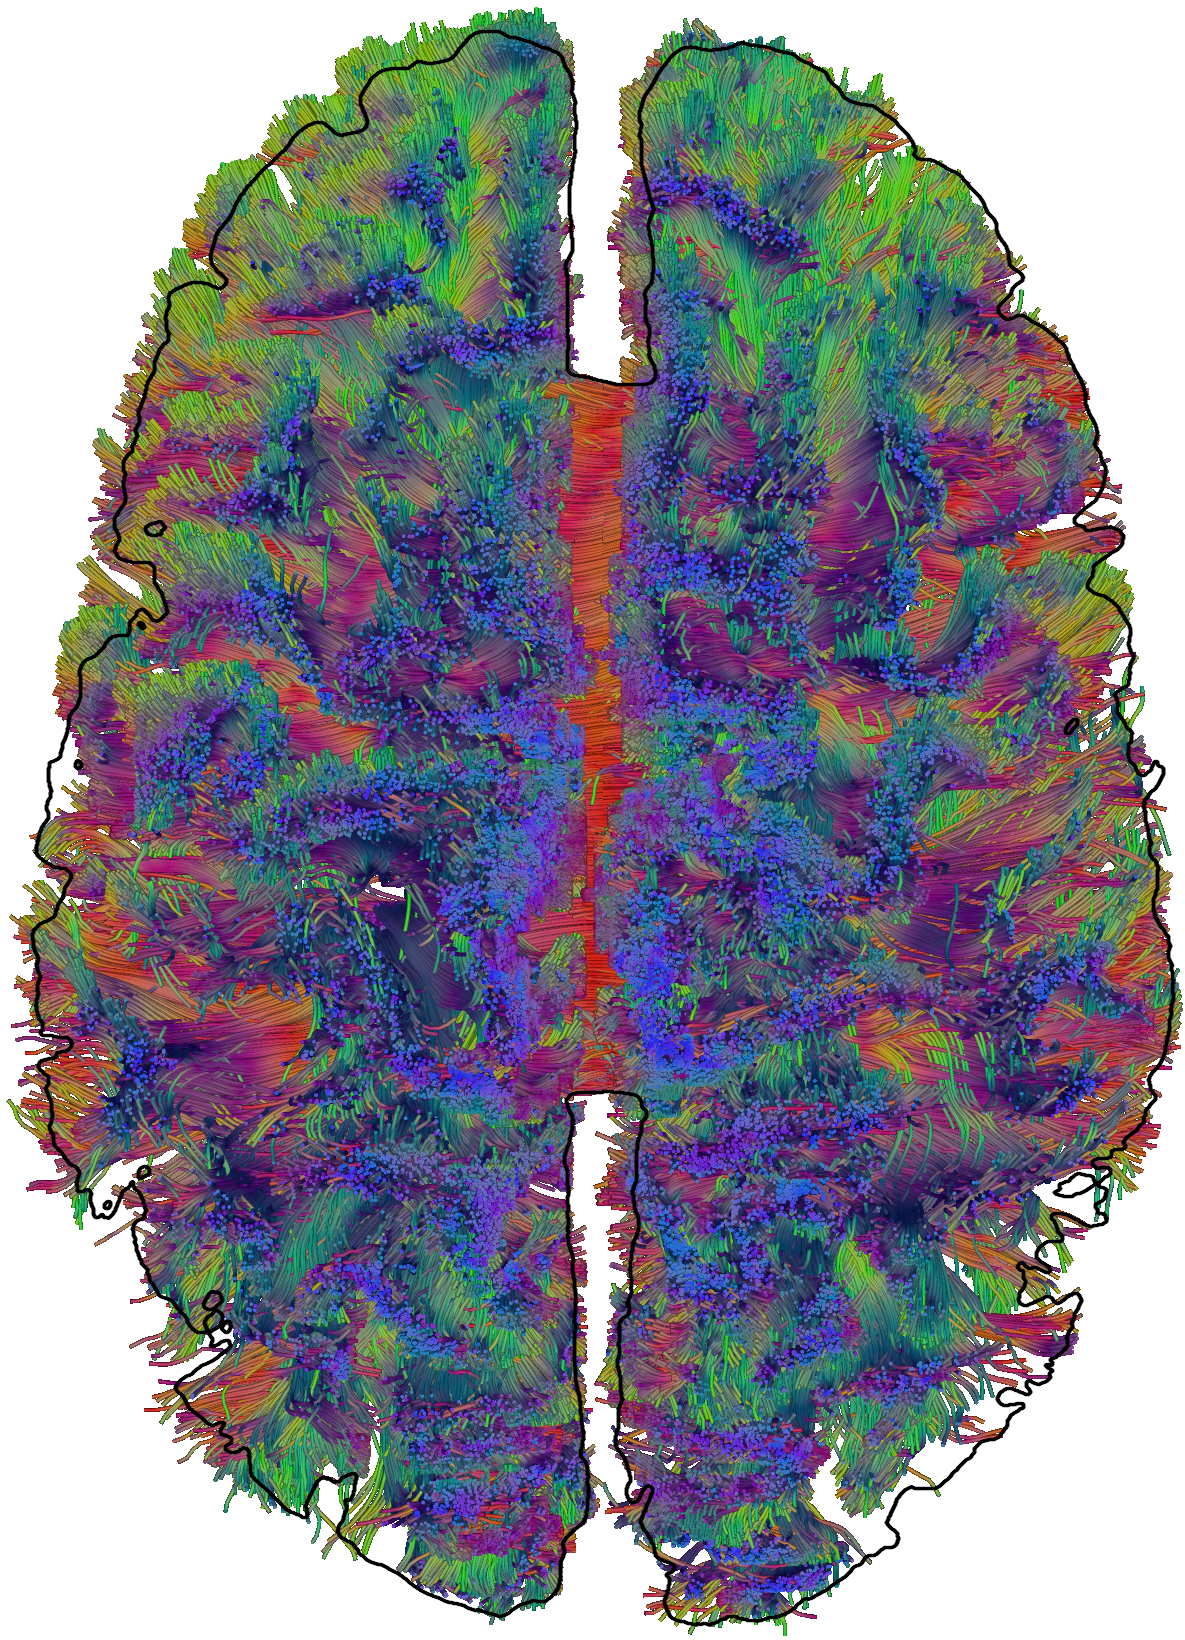
\includegraphics[width=\linewidth]{cc-sel-bootstrap-c}
		\caption{Consensus Selection Model}
\end{subfigure} 
\caption{Reconstruction of the corpus callosum Tract. The reconstruction within the
selection model misses a lot of the lateral spread. This gets greatly improved
within the consensus selection model. }
	\label{fig:CC}
\end{figure*}

As a first experiment we tract the right Cortiscospinal Tract (CST) from a seed
region, which is indicated with a dashed black line in Fig. \ref{fig:CST}. This tract is
known for its huge lateral spread, which is difficult to recover. The
novel proposed consensus approach increases the completeness of the lateral
spread especially for the selection model dramatically. While the selection
model is only able to recover a few single streamlines within this area the
consensus approach improves this area significantly. The consensus model also
improves the average and low-rank model. Here the spread is present in the base
model, but get denser by applying the consensus model. Further the streamlines
seems to be more aligned.

\begin{figure*}[h]
	\centering
	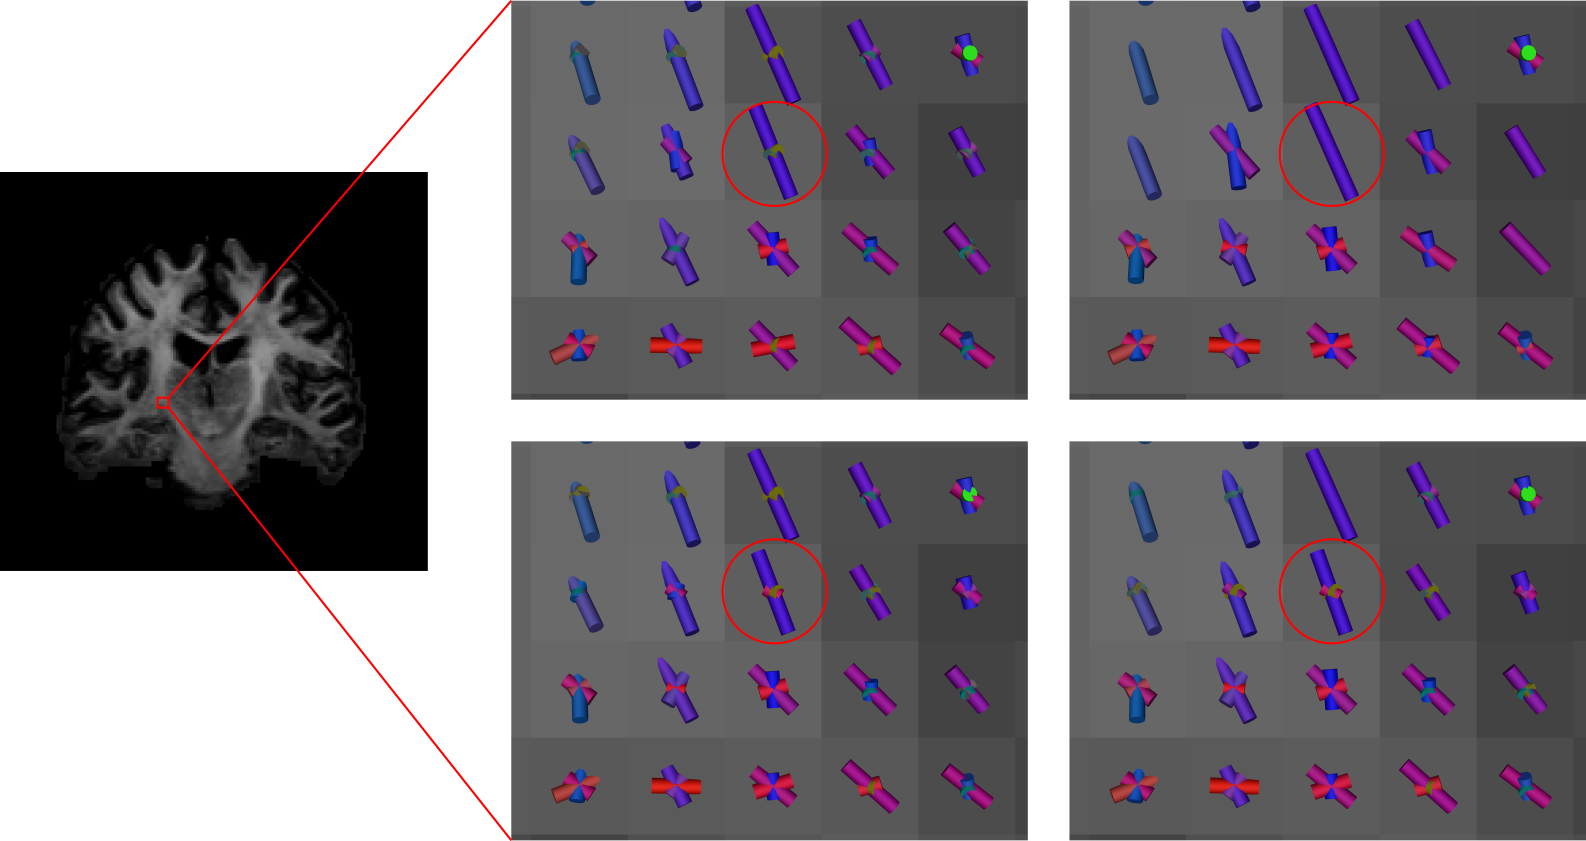
\includegraphics[width=\linewidth]{dir}
	\caption{Reconstructed fiber orientations of the different models, the
	red box in the left image denotes the position within the brain. Top row
shows models without consensus bootstrapping, bottom row with consensus
bootstrapping. Left: Averaging model. Right: selection model. Both consensus
models coincide in most voxels very well, although the base models differ as it
is visible in the red circled voxel.}
	\label{fig:directions}
\end{figure*}

This observation can be further explained by inspecting the multi vector fields
on Fig. \ref{fig:directions}. The most obvious difference between the average and
selection model is, that the average model has three fibers in
each voxel, while the selection model contains often just one fiber in a voxel.
For the tracking approach this leads to much more spread as seen in the
reconstruction of the CST. However, this also leads to much more 'fuzziness'
within the average model reconstruction. 
Applying the consensus to the average
and selection model leads to quiet similar multi vector fields as it can be seen
in the red circle. Within this voxel the average and selection model are
dissimilar but the consensus model agrees. This is also the case for the most
other voxels. However, in some voxels we see differences, as for example in the
voxel on top of the red circle where the average model contains $2$ fibers,
while the selection model contains just one fiber. Therefore, we conclude that
the consensus selection model and the average model are very similar, which is a
reason for the great improvement of the consensus selection model. 

\subsection{Quantitative Comparison}
\begin{figure}[t]
	\centering
	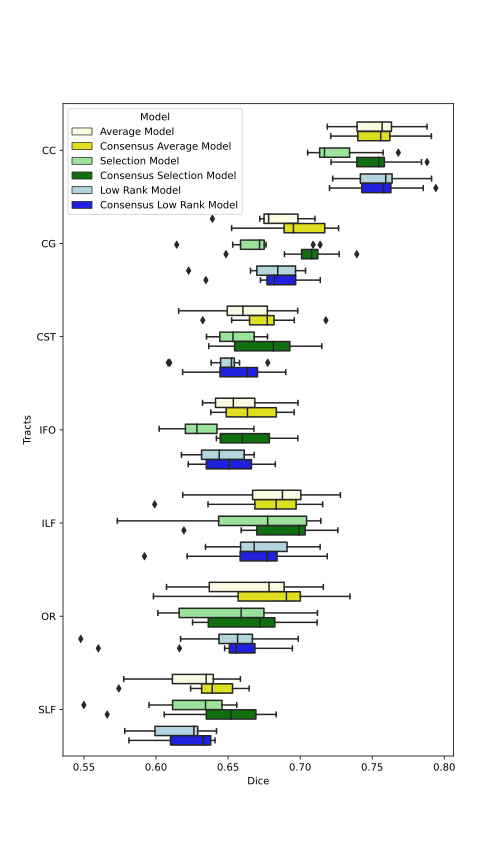
\includegraphics[width=\linewidth]{comparison-dice}
	\caption{Boxplots of the dice scores of all patients for all models. All
	subtracts are preprocessed separately, then merged and the dice scores
are calculated for a binary mask of the joint subtracts. The
average dice of the newly proposed consensus model is in all tracts greater or
equal to the dice score of the base model.}
	\label{fig:Dice}
\end{figure}

\begin{table*}
\centering
\begin{tabular}{p{4cm}p{1.5cm}p{1cm}p{1cm}p{1cm}p{1cm}}
	{}  & \rot{Consensus   Average  Model} & \rot{Selection Model} &
	\rot{Consensus Selection Model} & \rot{Low Rank Model} & \rot{Consensus
	Low Rank Model} \\ \hline  
Average Model &   {\cellcolor{lightgreen} 0.001} & {\cellcolor{lightred} 0.001}
& {\cellcolor{lightgreen} 0.002} & {\cellcolor{lightred} 0.001} & 0.063 \\
Consensus Average Model &   & {\cellcolor{lightred} 0.001} & 0.900 &
{\cellcolor{lightred} 0.001} & {\cellcolor{lightred} 0.001} \\
Selection Model &    & & {\cellcolor{lightgreen} 0.001} & 0.900 & 0.494 \\
Consensus Selection Model &  &  &  & {\cellcolor{lightred} 0.001} &
{\cellcolor{lightred} 0.001} \\
Low Rank Model &   &
 &   & & 0.494 \\
\end{tabular}
\caption{Comparison of different models by Nemenyi post-hoc test. All $p$ values
below $0.05$ are marked. If the top model is significantly better in green else
in red. The newly proposed base model shows for the selection and average model
and significant improvement. Also the average model is significantly better than
the selection and rank $3$ model, which supports our previous paper further.}
	\label{tab:sig}
\end{table*}


For a representative experiment we have reconstructed the corpus callosum (CC), the
cingulum (CG), the coricospinal tract (CST), the inferior fronto-occipital (IFO)
and the inferior longitudinal fasciculus (ILF), the optic radiation (OR), and
the superior longitudinal fasciculus (SLF). In the reference tragtographies, the
CC and SLF tracts were divided into subtracts, which we have merged into a single
tract. Further, we have merged the left and right parts of each tract. We have
evaluated the reconstruction quality by Dice score which is defined as
\[ 
	DICE = \frac{2 |RD \cap TR |}{|TR| + |RD|} ,
\]
where $RD$ denotes the reference data and $TR$ the tracking results
\cite{SCHILLING2019194}. A high Dice score is desired, as it denotes a high
overlap and a low overreach. To validate the results further, we applied a
Friedman test on model level to investigate if a model is significantly better
than any other model \cite{doi:10.1080/01621459.1937.10503522}. Post-hoc we
applied Nemenyi test to identify which models are significantly different
\cite{Nemenyi}.  


Figure \ref{fig:Dice} and Table \ref{tab:sig} summarize the results of our
quantitative comparison. In Fig. \ref{fig:Dice}, results from the average,
selection and low-rank model with and without use of the consensus model are
visualized using box plots to show the tract wise distribution of the Dice
scores. In Table \ref{tab:sig} the results of the post hoc Nemenyi tests are
shown. As a first result we denote that the Friedman test has shown that there
are significant differences between the models. 

To justify our previous work further, we are interested in the comparison of the
average, selection and low-rank model. The first impression from Fig.
\ref{fig:Dice} is that the average model is preferable to the other models and
that it depends on the tract if we prefer the selection or the low-rank model.
As it is visible in Table \ref{tab:sig} the improvement of the average model to
the other models is significant, while neither the selection model nor the
low-rank model is preferable to
the other. Therefore, we conclude that the average model, which we have proposed
within our last paper is significantly better than both other models. 

Within this work, we are more interested in the consensus model. Therefore, we
investigate if the improvement is significant between the model with and without
the application of the consensus. From Fig. \ref{fig:Dice} we can conclude, that
in 6 out of 7 tracts the consensus average model has an higher average Dice
score than the average model, that the consensus selection model has always an
higher Dice score, and that the consensus low-rank model has in 4 out of 7
tracts an higher Dice score. These changes are significant for the average and
selection model, while they are not significant for the low-rank model. 

Further, we want to compare the consensus models against each other. From Fig
\ref{fig:Dice} it seems that the consensus average and selection model are
preferable compared to the consensus low-rank model. Both models are equally
good compared by the mean dice score. This gets justified by the significance
tests. The consensus average as well as the consensus selection model are
significantly better than the consensus low-rank model. 

Overall we have shown that the consensus model improves our previously proposed
models significantly. However, the improvement by average Dice score is only for
the selection model large. 
\subsection{Computational Effort}
All experiments were computed on an Intel i9 with 3.3 GHz and 64 GB RAM. The
following durations are denoted in h:min:s or min:s.

The computation of a single bootstrap data sample took 1:10 on a single core,
multi-threaded fourth order fODF estimation took 4:33, the computation of the
selection model took 1:10, the computation of the averaging model took 1:30 and
the computation of the rank-3 model 0:40. The calculation of 100 bootstraps took
therefore 8:08:00, using all threads to create the bootstrap data as well as the
models. This also includes the computation of the consensus model, which on its
own took 11:00. The tracking itself is independent of the preprocessing steps.
It took approximately 3:30 for a bundle such it is shown in Figure
\ref{fig:Dice} on a single thread including postprocessing.  


